%%%%%%%%%%%%%%%%%%%%%%%%%%%%%%%%%%%%%%%%%%%%%%%%%%%%%%%%%%%%%%%%%%%%%%%%%%
%                                                                        %
%                            INTRODUCTION                                %
%                                                                        %
%%%%%%%%%%%%%%%%%%%%%%%%%%%%%%%%%%%%%%%%%%%%%%%%%%%%%%%%%%%%%%%%%%%%%%%%%%
\subsection*{}
\begin{frame}{Neutron - Gamma Discrimination}
  \begin{columns}[onlytextwidth]
    \begin{column}{0.45\textwidth}
    \large
    Methods of Neutron - Gamma Discrimination
    \normalsize
    \begin{itemize}
      \item Pulse shape 
      \item Pulse height
      \item Limit interactions
    \end{itemize}
    \end{column}
    \begin{column}{0.45\textwidth}
      How thick does a detector need to be to have less than one in a million interactions?
      \vspace{1cm}
      \begin{align*}
        \num{1E-6} &\le 1-\exp\left ( \frac{-\mu}{\rho}t \right )  
      \end{align*}
      \pause
      \huge
      \textcolor{red}{160 nm}
    \end{column}
  \end{columns}
\end{frame}
%%%%%%%%%%%%%%%%%%%%%%%%%%%%%%%%%%%%%%%%%%%%%%%%%%%%%%%%%%%%%%%%%%%%%%%%%%
\begin{frame}[t]{Pulse Height Discrimination}
  \begin{itemize}
    \item Use a lower lever discriminator to discard counts
    \item Mathematical Lower Lever Discriminator (MLLD)
  \end{itemize}
  \begin{columns}[onlytextwidth]
    \begin{column}{0.7\textwidth}
      \begin{figure}
          \vspace*{-1cm}
          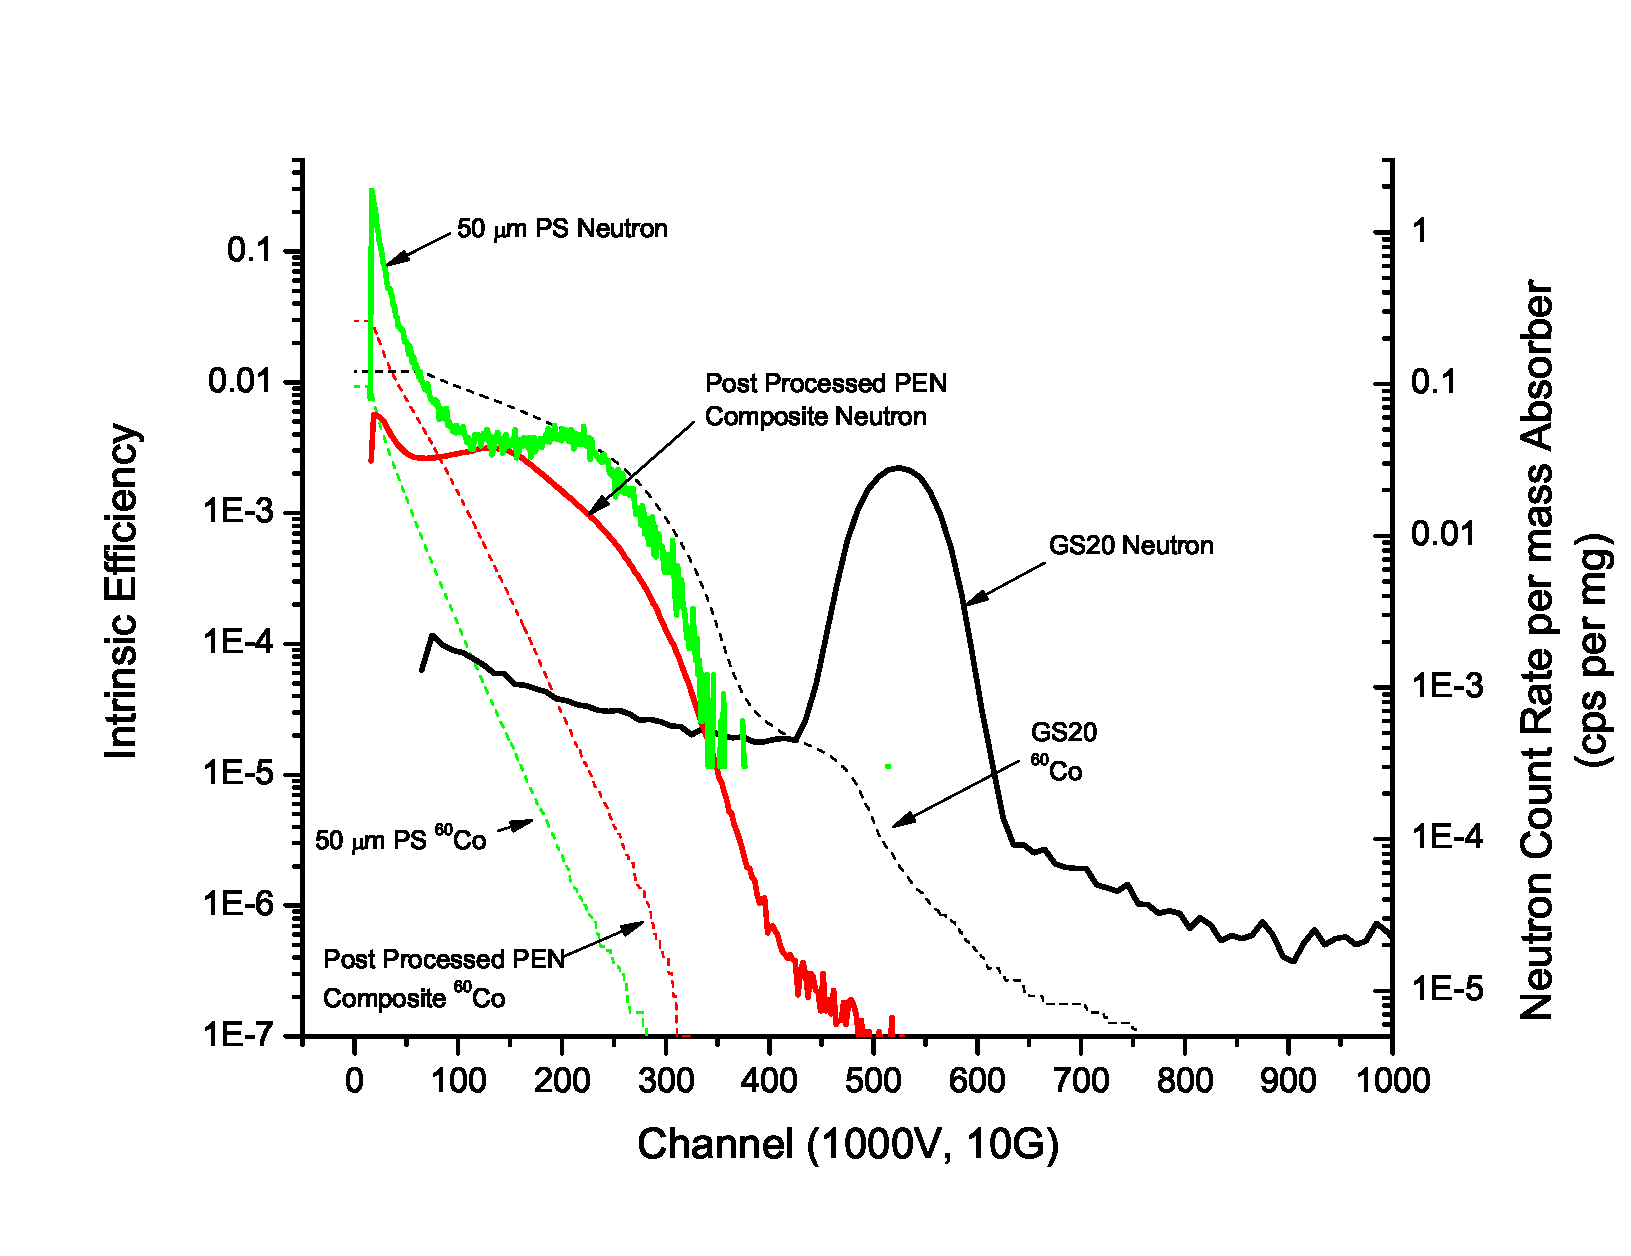
\includegraphics[width=\textwidth]{SC_UTDetectors_IntEff_CR}
      \end{figure}
    \end{column}
    \begin{column}{0.25\textwidth}
  \begin{align*}
    \frac{dL}{dx} = \frac{S_B\frac{dE}{dx}}{1+kB\frac{dE}{dx}}
  \end{align*}
    \end{column}
  \end{columns}
  Pulse height discrimination is equivalent to the energy deposition
\end{frame}
%%%%%%%%%%%%%%%%%%%%%%%%%%%%%%%%%%%%%%%%%%%%%%%%%%%%%%%%%%%%%%%%%%%%%%%%%%
%                                                                        %
%                             PROPOSED WORK                              %
%                                                                        %
%%%%%%%%%%%%%%%%%%%%%%%%%%%%%%%%%%%%%%%%%%%%%%%%%%%%%%%%%%%%%%%%%%%%%%%%%%
\subsection{Proposed Work}
\begin{frame}{Proposed Work}
  \large
  \centering{What is the optimal detector thickness?}
  \vspace{1cm}
  \normalsize
  \begin{itemize}
    \item Use GEANT4 to study the energy deposition in polymeric films
    \small
    \begin{itemize}
      \item How much energy is from the alpha, triton?
      \item How many and energy distribution of secondary electrons from neutrons, gammas
    \end{itemize}
    \item GEANT4 Simulations
    \begin{itemize}
      \item Single collision energy loss spectra
      \item Ranges of alpha, triton in material
      \item Simulated Spectra
    \end{itemize}
    \item Validate simulations with measurements
  \end{itemize}
\end{frame}
%%%%%%%%%%%%%%%%%%%%%%%%%%%%%%%%%%%%%%%%%%%%%%%%%%%%%%%%%%%%%%%%%%%%%%%%%%
%                                                                        %
%                               METHODS                                  %
%                                                                        %
%%%%%%%%%%%%%%%%%%%%%%%%%%%%%%%%%%%%%%%%%%%%%%%%%%%%%%%%%%%%%%%%%%%%%%%%%%
\subsection{Methods}
\begin{frame}[fragile]{GEANT4 Introduction}
What GEANT4 is:
\begin{itemize}
  \small
  \item \href{geant4.cern.ch}{geant4.cern.ch}
  \item Free software package for the simulation of the passage of particles through matter
  \item Essentially a collection of tools for geometry, materials, physics models, events and digitization, visualizations $\dots$
  \item Maintained by the CERN community, widely used in physics
\end{itemize}
What GEANT4 is not:
\begin{itemize}
  \small
  \item For the timid
  \begin{itemize}
    \item Users are responsible for correctly implementing their own physics
    \item Users are responsible for correctly implementing their own analysis
  \end{itemize}
  \item Stagnant - major release are still occurring
\end{itemize}
\end{frame}
%%%%%%%%%%%%%%%%%%%%%%%%%%%%%%%%%%%%%%%%%%%%%%%%%%%%%%%%%%%%%%%%%%%%%%%%%%
%                                                                        %
%                          PRELIMARY RESULTS                             %
%                                                                        %
%%%%%%%%%%%%%%%%%%%%%%%%%%%%%%%%%%%%%%%%%%%%%%%%%%%%%%%%%%%%%%%%%%%%%%%%%%
\subsection{Preliminary Results}
\begin{frame}{Single Collision Energy Loss Spectra}
  \begin{figure}
    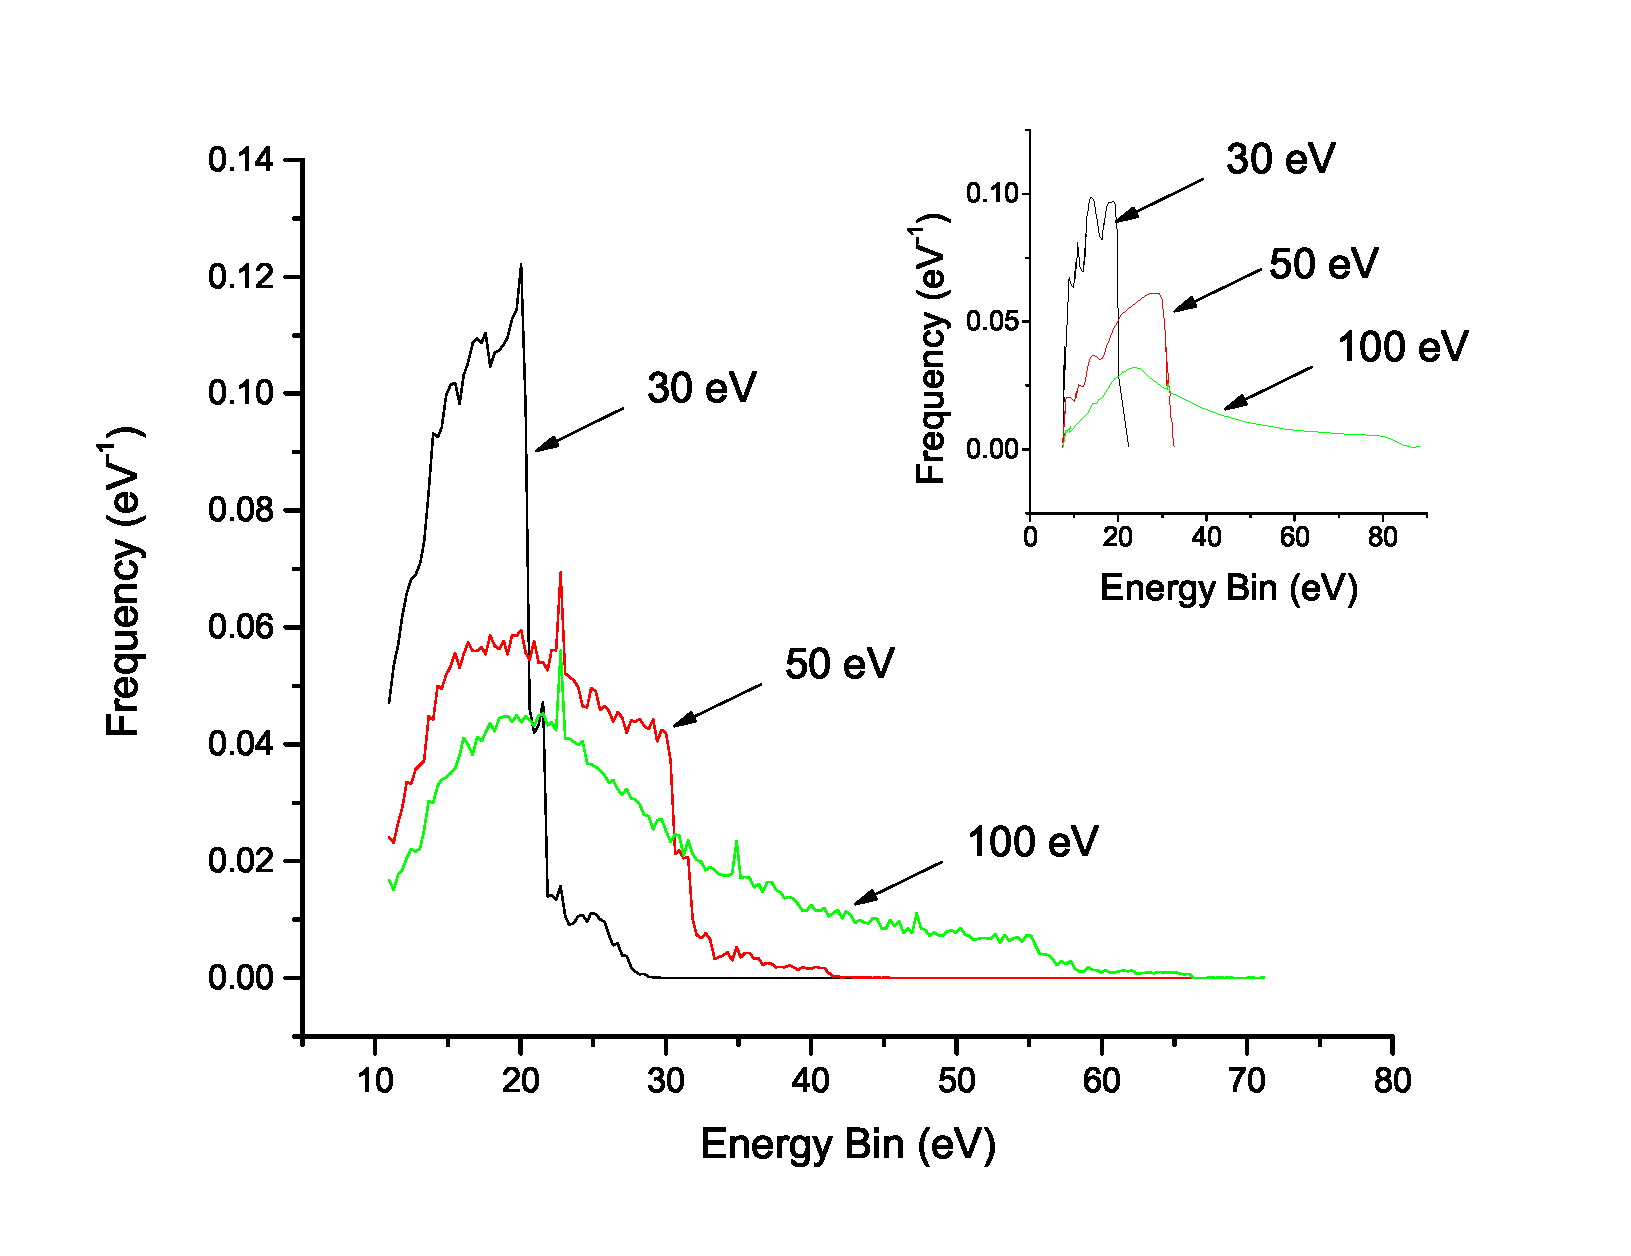
\includegraphics[width=\textwidth]{SingleCollsionEnergyLoss_Turner}
    \caption{Single Collision Energy Loss in Water\cite{turner_comparative_1982}}
  \end{figure}
\vspace{2mm}
Discrepancies are in the resolution of cross section data
\end{frame}
%%%%%%%%%%%%%%%%%%%%%%%%%%%%%%%%%%%%%%%%%%%%%%%%%%%%%%%%%%%%%%%%%%%%%%%%%%
\begin{frame}{Example Event}
  \begin{figure}
    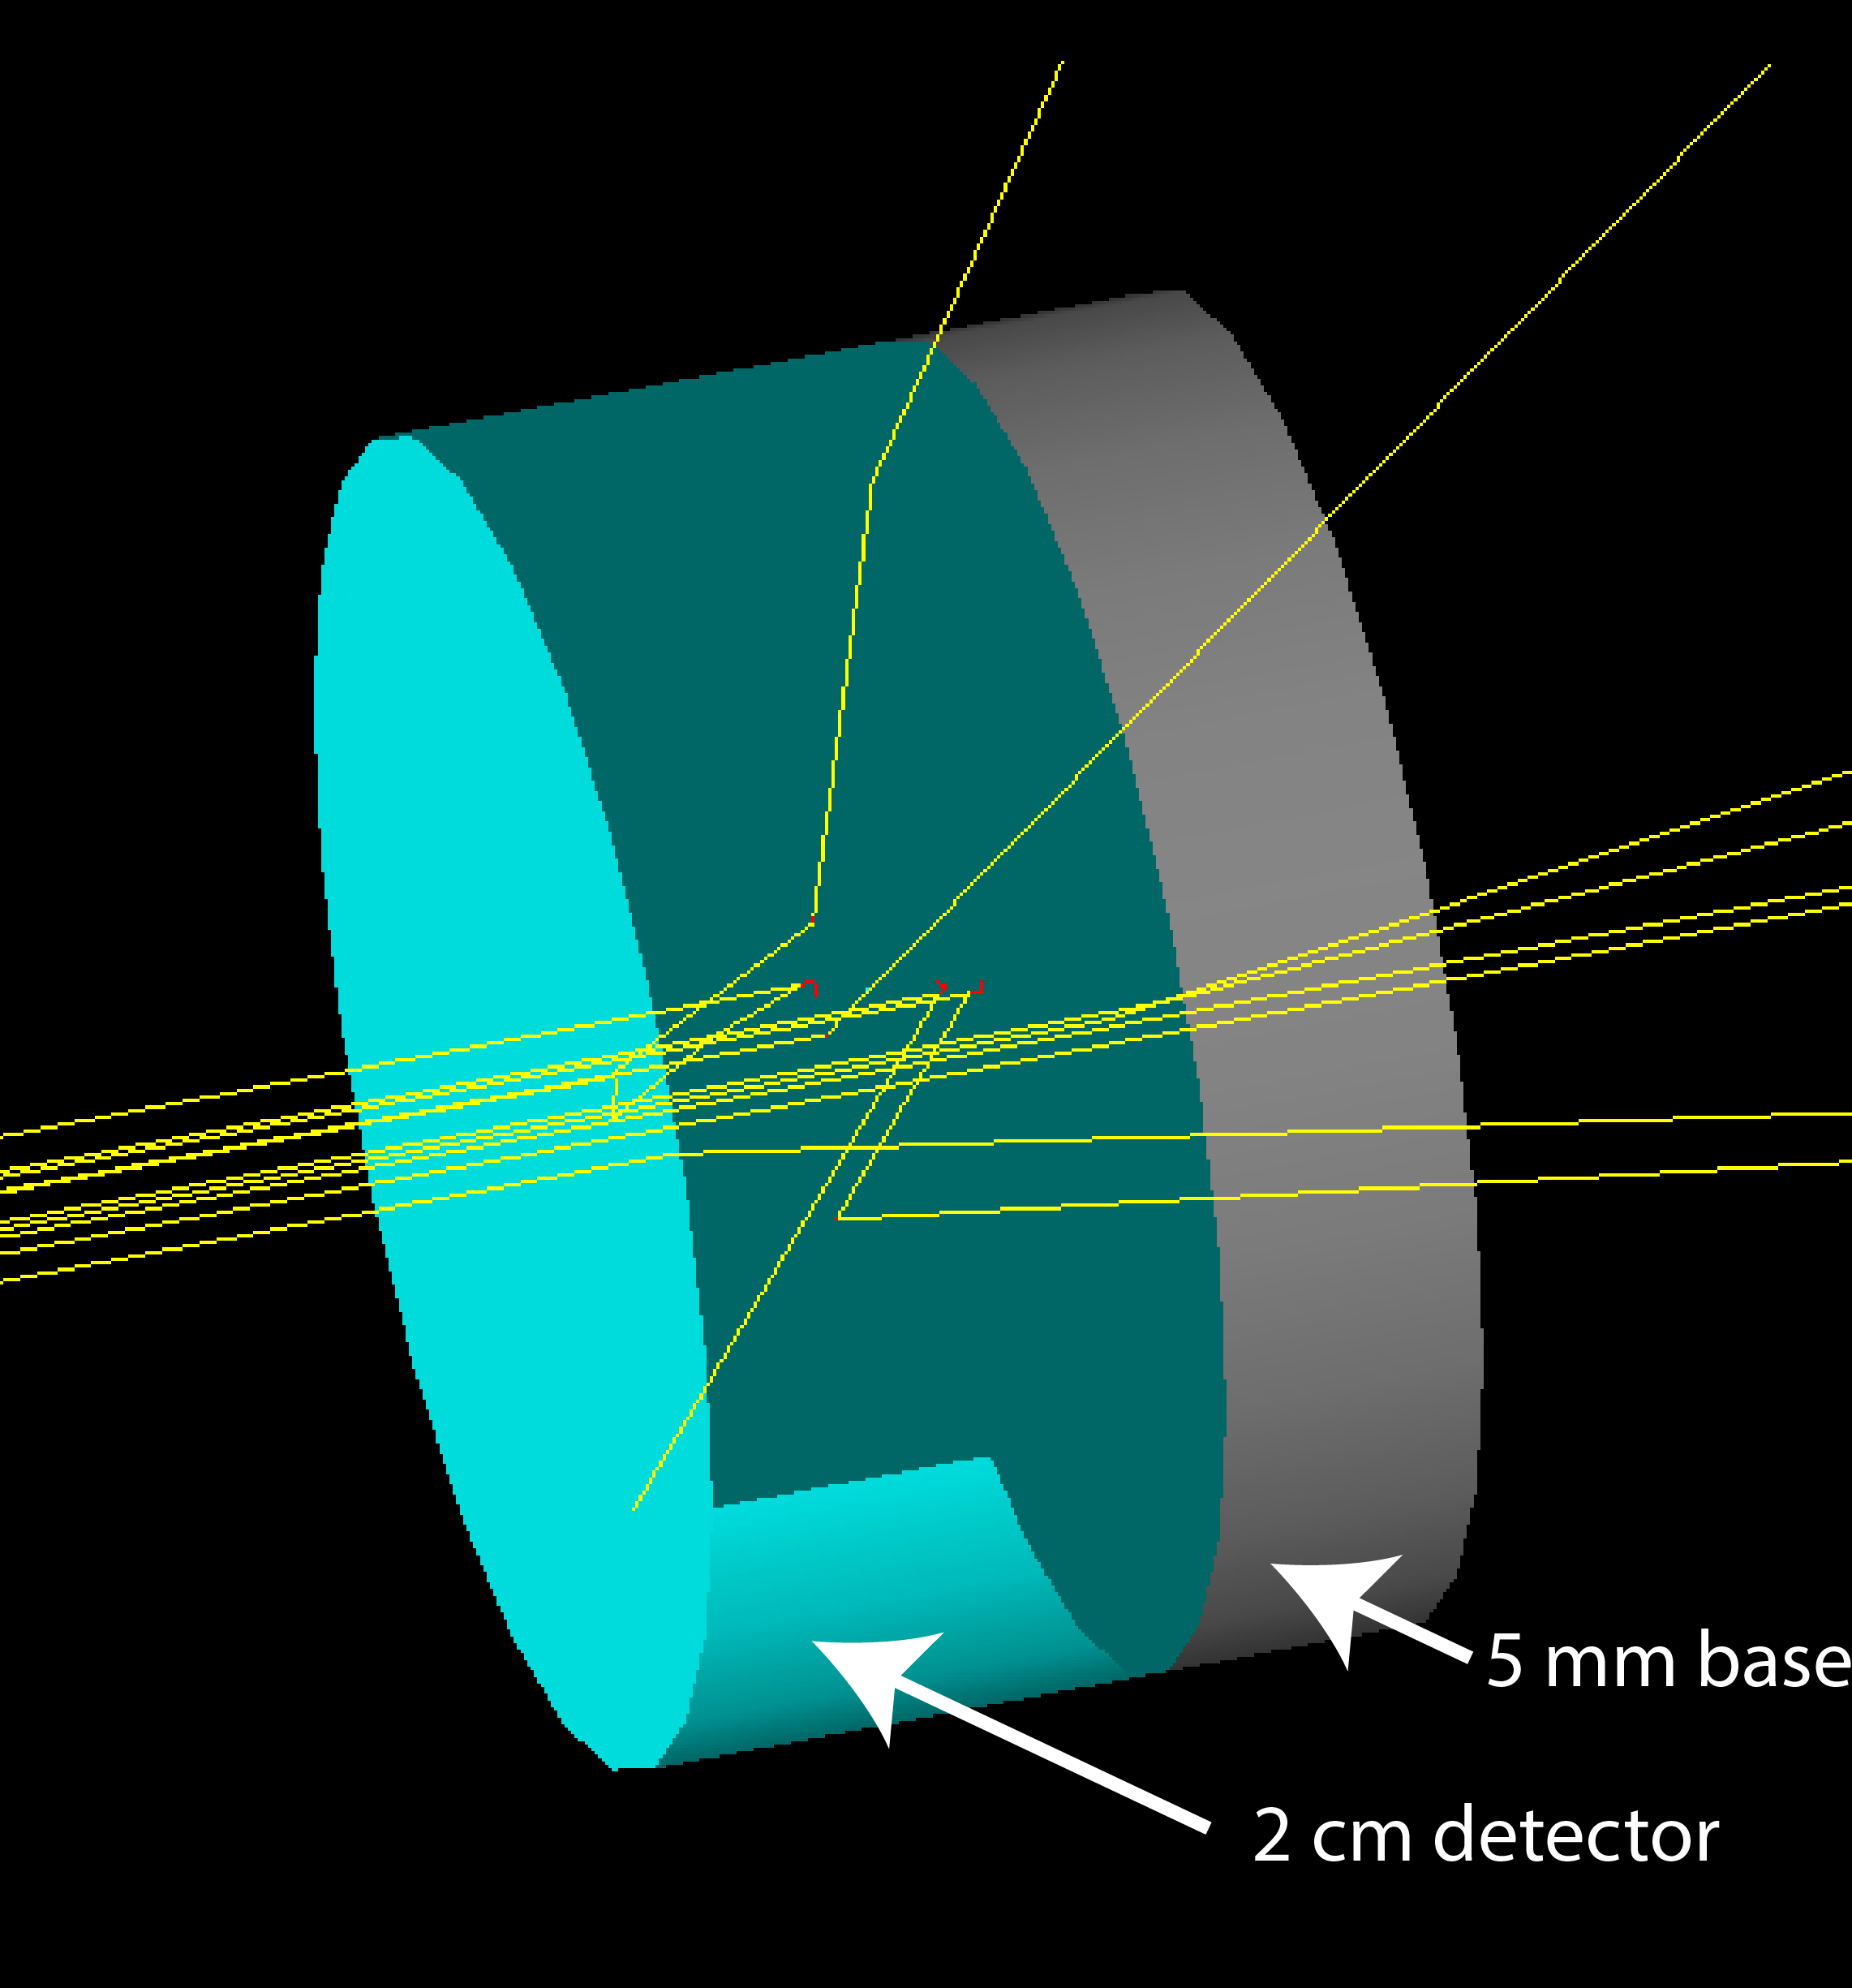
\includegraphics[height=0.75\textheight]{GEANT4AnnotatedGeo_EnergyDepEvent}
  \end{figure}
\end{frame}
%%%%%%%%%%%%%%%%%%%%%%%%%%%%%%%%%%%%%%%%%%%%%%%%%%%%%%%%%%%%%%%%%%%%%%%%%%
